\documentclass{standalone}
\usepackage{booktabs}
\usepackage{amsmath}
\usepackage{listings}
\usepackage{graphicx}
\usepackage{tabularx}
\newcommand{\exampleProgramSize}{4cm} 
\newcommand{\exampleTraceSize}{3.5cm}
\newcommand{\exampleDrawingSize}{1.25cm}
\lstset{basicstyle = \scriptsize\ttfamily}

\begin{document}
  \begin{tabular}{m{1.5cm}llc}
    \toprule
    \textbf{Drawing}&\textbf{Spec}&\textbf{Program}&%\begin{tabular}{c}
      \textbf{Compression factor}%\\\textbf{factor}
      %      \end{tabular}\\
      \\
    \midrule
    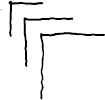
\includegraphics[width = \exampleDrawingSize]{figures/expert-29-trim.png}&
\begin{minipage}{\exampleTraceSize}\begin{lstlisting}
Line(2,15, 4,15)
Line(4,9, 4,13)
Line(3,11, 3,14)
Line(2,13, 2,15)
Line(3,14, 6,14)
Line(4,13, 8,13)
\end{lstlisting}
\end{minipage}&     \begin{minipage}{\exampleProgramSize} \begin{lstlisting}
for(i<3)
 line(i,-1*i+6,
      2*i+2,-1*i+6)
 line(i,-2*i+4,i,-1*i+6)
       \end{lstlisting}
     \end{minipage}&$\frac{6}{3} = 2\text{x}$\\\midrule
     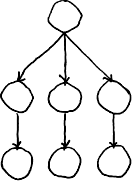
\includegraphics[width = \exampleDrawingSize]{figures/expert-52-trim.png}&
\begin{minipage}{\exampleTraceSize}\begin{lstlisting}
Line(5,13,2,10,arrow)
Circle(5,9)
Circle(8,5)
Line(2,8, 2,6,arrow)
Circle(2,5)
\end{lstlisting}
\small\emph{... etc. ...; 13 lines}
\end{minipage}&
             \begin{minipage}{\exampleProgramSize}\begin{lstlisting}
circle(4,10)
for(i<3)
 circle(-3*i+7,5)
 circle(-3*i+7,1)
 line(-3*i+7,4,-3*i+7,2,arrow)
 line(4,9,-3*i+7,6,arrow)
\end{lstlisting}
\end{minipage}&$\frac{13}{6} = 2.2\text{x}$\\\midrule
    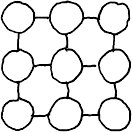
\includegraphics[width = \exampleDrawingSize]{figures/expert-38-trim.png}&
\begin{minipage}{\exampleTraceSize}\begin{lstlisting}
Circle(5,8)
Circle(2,8)
Circle(8,11)
Line(2,9, 2,10)
Circle(8,8)
Line(3,8, 4,8)
Line(3,11, 4,11)
\end{lstlisting}
  \small\emph{... etc. ...; 21 lines}
\end{minipage}&\begin{minipage}{\exampleProgramSize}
\begin{lstlisting}
for(i<3)
 for(j<3)
  if(j>0)
   line(-3*j+8,-3*i+7,
        -3*j+9,-3*i+7)
   line(-3*i+7,-3*j+8,
        -3*i+7,-3*j+9)
  circle(-3*j+7,-3*i+7)
\end{lstlisting}
\end{minipage}&$\frac{21}{6} = 3.5\text{x}$\\\midrule
\includegraphics[width = \exampleDrawingSize]{figures/expert-101-trim.png}&
\begin{minipage}{\exampleTraceSize}\begin{lstlisting}
Rectangle(1,10,3,11)
Rectangle(1,12,3,13)
Rectangle(4,8,6,9)
Rectangle(4,10,6,11)
\end{lstlisting}
  \small\emph{... etc. ...; 16 lines}
\end{minipage}&\begin{minipage}{\exampleProgramSize}
\begin{lstlisting}
for(i<4)
 for(j<4)
  rectangle(-3*i+9,-2*j+6,
            -3*i+11,-2*j+7)
\end{lstlisting}
\end{minipage}&$\frac{16}{3} = 5.3\text{x}$\\\midrule
%% 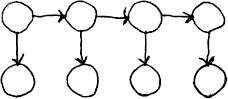
\includegraphics[width = \exampleDrawingSize]{figures/expert-75-extra-trim.png}&
%% \begin{minipage}{\exampleTraceSize}\begin{lstlisting}
%% Line(11,14,13,14,arrow)
%% Circle(10,10)
%% Line(10,13,10,11,arrow)
%% Circle(6,10)
%% \end{lstlisting}
%%     \small\emph{... etc. ...; 15 lines}
%% \end{minipage}&
%% \begin{minipage}{\exampleProgramSize}
%%     \begin{lstlisting}
%% for(i<4)
%%  line(-4*i+13,4,-4*i+13,2,arrow)
%%  for(j<3)
%%   if(j>0)
%%    circle(-4*i+13,4*j+-3)
%%   line(-4*j+10,5,-4*j+12,5,
%%        arrow)
%% \end{lstlisting}
%%   \end{minipage}&$\frac{15}{6} = 2.5\text{x}$\\\midrule    

  \includegraphics[width = \exampleDrawingSize]{figures/expert-71-trim.png}&
\begin{minipage}{\exampleTraceSize}\begin{lstlisting}
Line(3,10,3,14,arrow)
Rectangle(11,8,15,10)
Rectangle(11,14,15,15)
Line(13,10,13,14,arrow)
  \end{lstlisting}\small\emph{... etc. ...; 16 lines}%
  \end{minipage}&\begin{minipage}{\exampleProgramSize}
%% \begin{lstlisting}
%% for (i<3)
%%  circle(-3*i+7,1)
%%  circle(-3*i+7,6)
%%  line(-3*i+7,-1*i+4,-3*i+7,5)
%% \end{lstlisting}
\begin{lstlisting}
for(i<3)
 line(7,1,5*i+2,3,arrow)
 for(j<i+1)
  if(j>0)
   line(5*j-1,9,5*i,5,arrow)
  line(5*j+2,5,5*j+2,9,arrow)
 rectangle(5*i,3,5*i+4,5)
 rectangle(5*i,9,5*i+4,10)
rectangle(2,0,12,1)
\end{lstlisting}
\end{minipage}&$\frac{16}{9} = 1.8\text{x}$\\\midrule    

  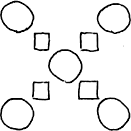
\includegraphics[width = \exampleDrawingSize]{figures/expert-72-trim.png}&

\begin{minipage}{\exampleTraceSize}\begin{lstlisting}
Circle(2,8)
Rectangle(6,9, 7,10)
Circle(8,8)
Rectangle(6,12, 7,13)
Rectangle(3,9, 4,10)
\end{lstlisting}\small\emph{... etc. ...; 9 lines}
  \end{minipage}&\begin{minipage}{\exampleProgramSize}
\begin{lstlisting}
reflect(y=8)
 for(i<3)
  if(i>0)
   rectangle(3*i-1,2,3*i,3)
  circle(3*i+1,3*i+1)
\end{lstlisting}
\end{minipage}&$\frac{9}{5} = 1.8\text{x}$ \\\bottomrule
  \end{tabular}
  \end{document}
